\chapter{Конструкторский раздел}
В этом разделе приводится подробное описание разрабатываемого метода, выделяются основные его компоненты, описываются метрики, оценивающие метод. В выводах аналитической части предлагается разработать новый метод распределения оперативной памяти приложений. Новый метод будет включать в себя выделение памяти запрашиваемого размера и ее освобождение.

\section{Структура программного комплекса}
\begin{figure}[!h]
	\begin{center}
		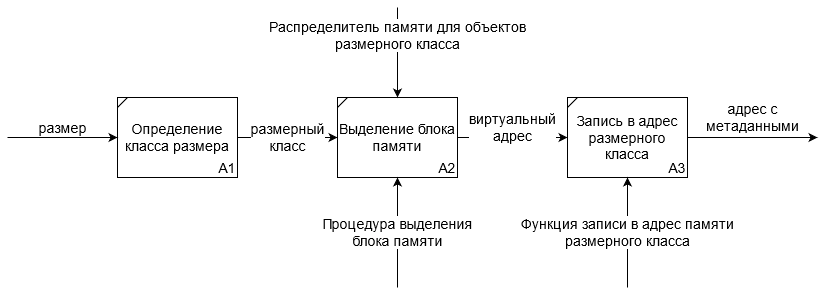
\includegraphics[scale=0.4]{images/block-allocation.png}
		\caption{Выделение блока памяти.}
		\label{block-allocation}
	\end{center}
\end{figure}

\begin{figure}[!h]
	\begin{center}
		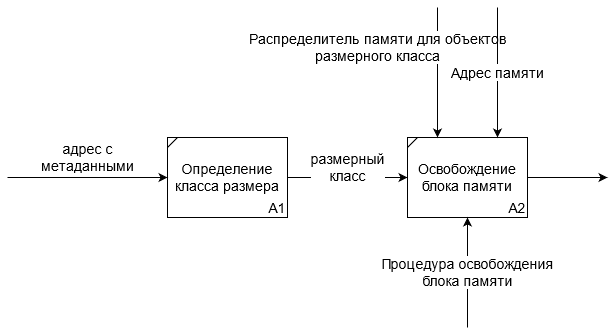
\includegraphics[scale=0.4]{images/block-free.png}
		\caption{Освобождение блока памяти.}
		\label{block-free}
	\end{center}
\end{figure}

Аллокатору передается размер памяти, которую необходимо выделить, в байтах. Далее, в зависимости от того, к какому классу относится размер, есть три варианта выделения памяти:
\begin{itemize}
	\item малые объекты, это объекты размер кототрых менее либо равен 2048-и байтам, они выделяются через специализированный аллокатор для малых объектов;
	\item большие объекты, это объекты размер которых менее либо равен 1МБ по умолчанию, (ограничение может быть изменено, но не должно превышать 268431360 байт) они выделяются через аллокатор для больших объектов;
	\item огромные объекты, класс объектов, размер которых более чем ограничение для больших объектов, такие объекты выделяются сразу через систменый вызов \textbf{mmap}.
\end{itemize}

Результатом запроса в распределитеть памяти является адрес, выровненный по размеру страницы и содержащий в себе всю необходимую информацию для освобождения объекта. После освобождения, память кэшируется в случае для малых и больших запросов. Память под огромные объекты, при освобождениии, сразу возвращается ОС.

\subsection{Основная идея}
Метод основан на использовании старших бит виртуального адреса. На рисунке \ref{64bit-memory-addressing} показана диаграмма перевода виртульного адреса в физический в 64-ъ битной системе.

\begin{figure}[!h]
	\begin{center}
		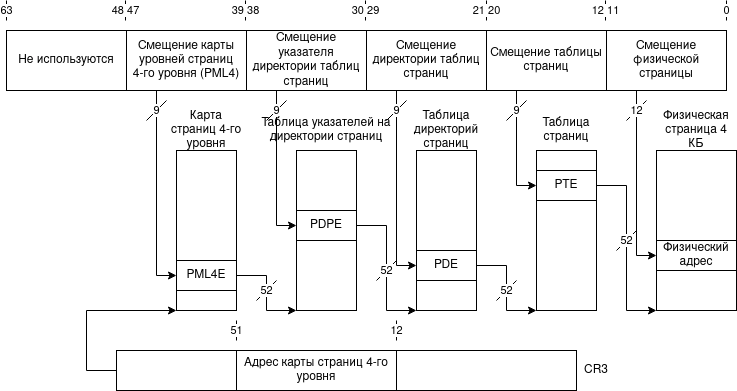
\includegraphics[scale=0.6]{images/64bit-memory-addressing.png}
		\caption{Адресация памяти в 64-х битном режиме.}
		\label{64bit-memory-addressing}
	\end{center}
\end{figure}

Как видно из рисунка \ref{64bit-memory-addressing}, для адресации используются только первые 48 бит из 64-х, остальные 16 бит разграничивают виртуального адресное пространство на зоны нижних и верхних адресов. Биты 63-48 разграничивают знак, если 47-й выставлен в 0, то все верхние 16 тоже выставлены в 0 и такие адреса относятся к нижней половине, если 47-й бит выставлен в 1, то биты 63-48 тоже равны 1 и такие адреса относятся к верхней половине виртульных адресов.

\begin{figure}[!h]
	\begin{center}
		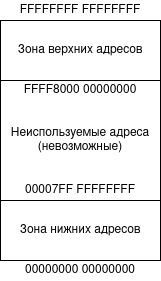
\includegraphics[scale=0.6]{images/48bit-half-spaces.png}
		\caption{48-и битная адресация.}
		\label{48bit-half-spaces}
	\end{center}
\end{figure}

Данная реализация распределителся памяти использует верхние 16 бит виртуального 64-х битного адреса для хранения информации о типе (большой/малый) и размерном классе объекта.

\subsection{Аллокатор для малых объектов}

\subsection{Аллокатор для больших объектов}

\subsection{Аллокатор для огромных объектов}